% Page de garde du rapport
\title{\Large \textbf{Mémoire de projet Master 2}\\[0.2cm] 
\Huge \textbf{AI Engine of OpenSource Together}}
\date{\Large Année scolaire 2025–2026}
\author{\Large Djebali Hicham}

\maketitle

\begin{figure}[H]
  \centering
  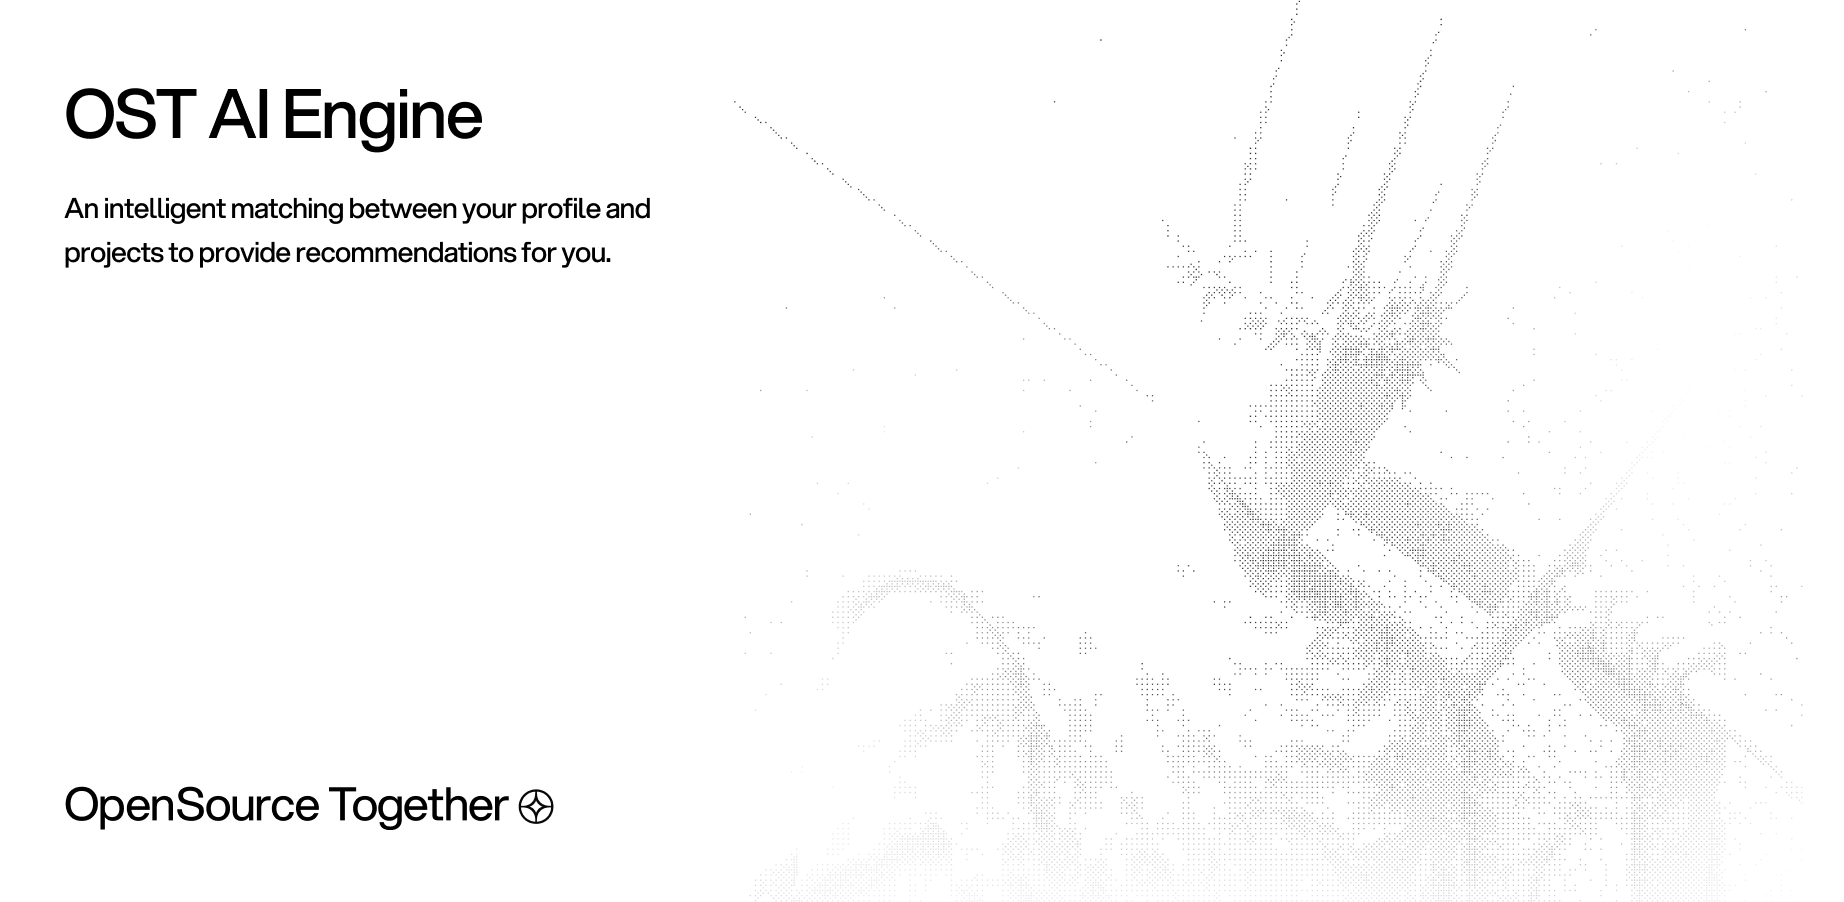
\includegraphics[width=1\linewidth]{images/ost-knight.png}
  \caption*{Illustration : OST Knight}
\end{figure}

\vspace{1cm}

\noindent\textbf{Résumé}

\begin{justify}
Ce mémoire présente l’AI Engine d’\href{https://opensource-together.com/}{OpenSource Together}, une plateforme collaborative née d’une équipe passionnée sur $\mathbb{X}$ pour dynamiser l’open source européen. J’y ai conçu un système de recommandation innovant, basé sur une infrastructure data et IA, capable de proposer régulièrement des projets tendances et des recommandations personnalisées selon chaque profil. Ce projet inédit allie rigueur technique et esprit communautaire, avec pour ambition de bâtir une communauté où la passion et l’innovation priment.
\end{justify}

\vspace{1cm}

\begin{flushleft}
  
\includegraphics[width=0.08\linewidth]{images/logo-datascientest.png}
  \hspace{1cm}
  \raisebox{0.35cm}{
\includegraphics[width=0.3\linewidth]{images/logo-opensource-together.png}}
\end{flushleft}
